%% ============================================================
%% EJ-204 vs EJ-230 Bar — TIR-only timing resolution study
%% Geant4 11.4 MT Simulation | rrios / dowiyogo@gmail.com
%% ============================================================
\documentclass[aspectratio=169,10pt]{beamer}

\usetheme{Boadilla}
\usecolortheme{seahorse}
\useinnertheme{circles}
\setbeamertemplate{navigation symbols}{}
\setbeamertemplate{footline}[frame number]

\usepackage[utf8]{inputenc}
\usepackage[T1]{fontenc}
\usepackage{lmodern}
\usepackage{booktabs}
\usepackage{siunitx}
\usepackage{xcolor}
\usepackage{graphicx}
\usepackage{tikz}
\usetikzlibrary{shapes.geometric,arrows.meta,decorations.pathmorphing,patterns,calc}

%% Images live in the build output directory
\graphicspath{{../build_t0minidaq/}}

% ── Colors ───────────────────────────────────────────────────────────────────
\definecolor{ej204col}{RGB}{30,80,180}    % blue: EJ-204
\definecolor{ej230col}{RGB}{180,50,20}    % red:  EJ-230
\definecolor{scintgr}{RGB}{60,160,60}     % scintillator green
\definecolor{sipmcol}{RGB}{30,30,180}     % SiPM blue
\definecolor{muoncol}{RGB}{180,0,0}       % muon red
\definecolor{airgap}{RGB}{200,230,255}    % light blue: air

% ── Title ────────────────────────────────────────────────────────────────────
\title[EJ-204 vs EJ-230 Bar -- TIR-only]%
      {Timing Resolution: EJ-204 vs EJ-230\\
       on a Plastic Scintillator Bar --- TIR-only Configuration}

\subtitle{Geant4 11.4 MT Simulation ---
          \texttt{feat/ej204-bar-tir-only} \& \texttt{feat/ej230-bar-tir-only}}

\author{R.~Rios}
\institute{Simulated using \texttt{ej200} framework (SSLG4)}
\date{\today}

% ─────────────────────────────────────────────────────────────────────────────
\begin{document}

\begin{frame}
  \titlepage
\end{frame}

% ─────────────────────────────────────────────────────────────────────────────
\section{Detector Geometry}

\begin{frame}{Detector Geometry --- EJ-204/EJ-230 Scintillator Bar}

\begin{columns}[T]
  %% ── Left: TikZ schematic ─────────────────────────────────────────────────
  \begin{column}{0.58\textwidth}
  \centering
  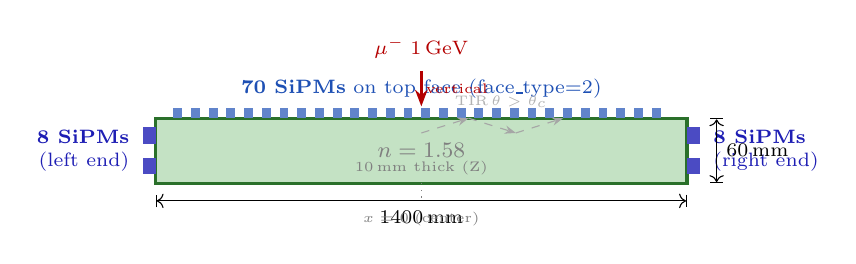
\begin{tikzpicture}[scale=0.75, every node/.style={font=\scriptsize}]

    %% Bar body (schematic: X along bar length, Y = height)
    \fill[scintgr!30] (0,-0.55) rectangle (9.0,0.55);
    \draw[scintgr!70!black, very thick] (0,-0.55) rectangle (9.0,0.55);

    %% End SiPMs -- left (face_type=0)
    \fill[sipmcol!80] (-0.22,-0.40) rectangle (0,-0.12);
    \fill[sipmcol!80] (-0.22, 0.12) rectangle (0, 0.40);
    \node[left, sipmcol, align=right] at (-0.28, 0)
      {\textbf{8 SiPMs}\\(left end)};

    %% End SiPMs -- right (face_type=1)
    \fill[sipmcol!80] (9.0,-0.40) rectangle (9.22,-0.12);
    \fill[sipmcol!80] (9.0, 0.12) rectangle (9.22, 0.40);
    \node[right, sipmcol, align=left] at (9.28, 0)
      {\textbf{8 SiPMs}\\(right end)};

    %% Top SiPMs (face_type=2) -- strip along top face
    \foreach \x in {0.3,0.6,...,8.7} {
      \fill[ej204col!70] (\x, 0.55) rectangle (\x+0.15, 0.72);
    }
    \node[above, ej204col] at (4.5, 0.72)
      {\textbf{70 SiPMs} on top face (face\_type=2)};

    %% Muon arrow (vertical, entering from top at bar center)
    \draw[muoncol, very thick, -{Stealth[length=6pt]}]
      (4.5, 1.35) -- (4.5, 0.75);
    \node[above, muoncol] at (4.5, 1.4) {$\mu^-$\;1\,GeV};
    \node[muoncol] at (5.1, 1.05) {\tiny vertical};

    %% Critical angle indication (dashed TIR ray)
    \draw[dashed, gray!70, -{Stealth[length=4pt]}]
      (4.5, 0.3) -- (5.3, 0.55);
    \draw[dashed, gray!70, -{Stealth[length=4pt]}]
      (5.3, 0.55) -- (6.1, 0.30);
    \draw[dashed, gray!70, -{Stealth[length=4pt]}]
      (6.1, 0.30) -- (6.9, 0.55);
    \node[gray!60, above] at (5.85, 0.56)
      {\tiny TIR\,$\theta>\theta_c$};

    %% Dimension labels
    \draw[|<->|, thin] (0,-0.85) -- (9.0,-0.85)
      node[midway, below] {\SI{1400}{mm}};
    \draw[|<->|, thin] (9.5,-0.55) -- (9.5,0.55)
      node[midway, right] {\SI{60}{mm}};
    \node[gray] at (4.5, 0) {\footnotesize $n=1.58$};
    \node[gray] at (4.5,-0.3) {\tiny \SI{10}{mm} thick (Z)};

    %% Center marker
    \draw[dotted, gray] (4.5,-0.55) -- (4.5,-0.85);
    \node[below, gray] at (4.5,-0.88) {\tiny $x=0$\;(center)};

  \end{tikzpicture}

  \vspace{0.3em}
  {\footnotesize XY side view (not to scale in Y)}
  \end{column}

  %% ── Right: parameter table ────────────────────────────────────────────────
  \begin{column}{0.40\textwidth}
  \small
  \begin{block}{Bar Geometry}
    \begin{tabular}{@{}ll@{}}
      Shape        & Rectangular bar \\
      Length       & \SI{1400}{mm} \\
      Height       & \SI{60}{mm} \\
      Width        & \SI{10}{mm} \\
      Refractive index & $n = 1.58$ \\
      TIR angle    & $\theta_c = 39.3^\circ$ \\
    \end{tabular}
  \end{block}

  \begin{block}{Readout}
    \begin{tabular}{@{}ll@{}}
      End SiPMs   & 8 per end, 2 ends \\
      Top SiPMs   & 70 (face\_type=2) \\
      Total       & 86 SiPMs \\
      Coupling    & polished, direct \\
    \end{tabular}
  \end{block}

  \begin{block}{Surface (TIR-only)}
    \begin{tabular}{@{}ll@{}}
      Type        & Polished, dielectric \\
      Reflector   & \textbf{none} (bare air) \\
      $\theta>\theta_c$ & 100\% TIR \\
      $\theta<\theta_c$ & Fresnel, mostly lost \\
    \end{tabular}
  \end{block}
  \end{column}
\end{columns}

\end{frame}

% ─────────────────────────────────────────────────────────────────────────────
\begin{frame}{Two Scintillators Compared}

\begin{columns}[T]

  \begin{column}{0.48\textwidth}
  \begin{alertblock}{\textcolor{ej204col}{\textbf{EJ-204 (OPSC-101)}}}
    \begin{tabular}{@{}ll@{}}
      Decay time  & \SI{2.1}{ns} \\
      Rise time   & \SI{0.5}{ns} \\
      Light yield & \SI{10000}{ph/MeV} \\
      Att. length & \SI{160}{cm} \\
      Peak $\lambda$ & \SI{408}{nm} \\
    \end{tabular}\\[0.4em]
    \textbf{Branch:} \texttt{feat/ej204-bar-tir-only}
  \end{alertblock}
  \end{column}

  \begin{column}{0.48\textwidth}
  \begin{alertblock}{\textcolor{ej230col}{\textbf{EJ-230 (OPSC-106)}}}
    \begin{tabular}{@{}ll@{}}
      Decay time  & \SI{1.5}{ns} \\
      Rise time   & \SI{0.5}{ns} \\
      Light yield & \SI{9200}{ph/MeV} \\
      Att. length & \SI{120}{cm} \\
      Peak $\lambda$ & \SI{391}{nm} \\
    \end{tabular}\\[0.4em]
    \textbf{Branch:} \texttt{feat/ej230-bar-tir-only}
  \end{alertblock}
  \end{column}

\end{columns}

\vspace{0.7em}

\begin{block}{Simulation Parameters (identical for both)}
  \centering
  \begin{tabular}{@{}lllll@{}}
    \toprule
    Particle & Energy & Direction & Position & Statistics \\
    \midrule
    $\mu^-$ & \SI{1}{GeV} & vertical ($-Y$) & $x=0$ (bar centre) & 5000 events \\
    \bottomrule
  \end{tabular}
\end{block}

\vspace{0.3em}
{\footnotesize
GROUPVEL aliasing fix applied: world air set to $v_g = c/1.58$.
SiPM electronics jitter: $\sigma_\text{jitter}=0$ (intrinsic photon limit).
Readout mode: \texttt{EndTop} (end + top SiPMs simultaneously active).
}

\end{frame}

% ─────────────────────────────────────────────────────────────────────────────
\section{Simulation Results}

\begin{frame}{Photon Yield per Event --- Top vs.\ End SiPMs}

\begin{columns}[T]

  \begin{column}{0.52\textwidth}
  \begin{block}{Mean $\langle N_\text{pe}\rangle$ per event}
  \renewcommand{\arraystretch}{1.3}
  \begin{tabular}{@{}lSS@{}}
    \toprule
    SiPM group & {\textbf{EJ-204}} & {\textbf{EJ-230}} \\
    \midrule
    Top SiPMs (70, face\_type=2)  & 117.1 & 106.2 \\
    Left end (8, face\_type=0)    & 0.39  & {$\sim\!0.4$} \\
    Right end (8, face\_type=1)   & 0.38  & {$\sim\!0.4$} \\
    \midrule
    Top / End ratio & \multicolumn{2}{c}{$\sim 300\times$} \\
    \bottomrule
  \end{tabular}
  \end{block}
  \end{column}

  \begin{column}{0.46\textwidth}
  \begin{alertblock}{Key result: end SiPMs are blind}
  \small
  Without Mylar/Vikuiti reflector, photons must travel \SI{700}{mm}
  to reach the end SiPMs.
  Each lateral bounce has a chance of escaping TIR ($\theta < 39.3^\circ$
  from normal $\to$ Fresnel loss).
  After $\sim\!700$ mm of propagation:
  \begin{itemize}\setlength\itemsep{0.1em}
    \item Bulk absorption: $e^{-700/1600} \approx 0.64$
    \item Accumulated TIR escape losses $\to$ only $\sim\!0.4$\,ph reach each end
  \end{itemize}
  \textbf{Top SiPMs are the only viable readout} for TIR-only timing.
  \end{alertblock}
  \end{column}
\end{columns}

\vspace{0.5em}
{\footnotesize
Light yield ratio: EJ-204/EJ-230 = $117.1/106.2 = 1.10$, consistent with
light-yield ratio $10000/9200 = 1.087$ from material tables.
}

\end{frame}

% ─────────────────────────────────────────────────────────────────────────────
\section{Timing Resolution}

\begin{frame}{Timing Resolution Setup --- $k$-th Photon Order Statistics}

\begin{columns}[T]
  \begin{column}{0.56\textwidth}
  \begin{block}{Method}
    \begin{enumerate}\setlength\itemsep{0.25em}
      \item Per event: sort all photon arrival times on the \textbf{top SiPMs}
            (70 SiPMs combined).
      \item Extract $t_{(k)}$ = $k$-th earliest arrival time.
      \item Build histogram of $t_{(k)}$ across all 5000 events.
      \item Fit Gaussian to the core ($\pm 2\sigma_{68\%}$ range) ---
            robust against the right-skew of order statistics.
      \item $\sigma(k)$ = Gaussian width = timing resolution when
            triggering on the $k$-th photon.
    \end{enumerate}
  \end{block}

  \vspace{0.4em}
  \begin{block}{Why $\sigma(k)$ is expected to be monotonically increasing}
  \small
  \begin{tabular}{@{}l@{$\;\Rightarrow\;$}l@{}}
    $k=1$ & fastest photon; dominated by transit geometry\\
    $k\uparrow$ & deeper into scintillation time dist.\ $\to$ wider $\sigma$ \\
    No dip & unlike cylinder: no direct/reflected photon cross-over \\
  \end{tabular}
  \end{block}
  \end{column}

  \begin{column}{0.42\textwidth}
  \begin{block}{Timing components at top SiPMs}
  \small
  \begin{enumerate}\setlength\itemsep{0.2em}
    \item \textbf{Emission time}: exponential $\tau_\text{decay}$
          (dominant at \SI{2.1}{ns} / \SI{1.5}{ns})
    \item \textbf{Transit time}: $\sim$\SI{30}{mm} mean vertical path
          $\to \sigma_\text{tr} \approx \SI{30}{ps}$ spread
    \item \textbf{TIR path variance}: photons bouncing laterally
          add a few \si{ps} of extra spread
  \end{enumerate}

  \vspace{0.4em}
  \begin{tabular}{@{}lS[table-format=3.0]@{}}
    \toprule
    Config & {$\langle N_\text{pe}\rangle$ top} \\
    \midrule
    EJ-204 & 117 \\
    EJ-230 & 106 \\
    \bottomrule
  \end{tabular}
  \end{block}
  \end{column}
\end{columns}

\end{frame}

% ─────────────────────────────────────────────────────────────────────────────
\begin{frame}{$\sigma(k)$ vs $k$ --- Timing Resolution Curves}

  \begin{center}
    \includegraphics[width=0.60\textwidth]{bar_timing_sigma_vs_k.png}
  \end{center}

  \vspace{-0.5em}
  {\footnotesize
  \textcolor{ej204col}{\textbf{Blue (EJ-204)}}: $\sigma_\text{Gauss}$ (filled circles) and
  $\sigma_\text{IQR}$ (dashed).
  \textcolor{ej230col}{\textbf{Red (EJ-230)}}: same estimators.
  Both curves rise monotonically: $k_\text{opt}=2$ for both configurations.
  EJ-230 is consistently $\sim\!15\%$ better across all $k$ values.
  }

\end{frame}

% ─────────────────────────────────────────────────────────────────────────────
\begin{frame}{$t_{(k)}$ Distributions --- Gaussian Fits (top SiPMs)}

  \begin{center}
    \includegraphics[width=0.72\textwidth]{bar_timing_fits_panels.png}
  \end{center}

  \vspace{-0.3em}
  {\footnotesize
  Each panel: $\Delta t_k = t_{(k)} - \mathrm{median}(t_{(k)})$ across 5000 events.
  Solid curve: EJ-204 (\textcolor{ej204col}{blue}); dashed: EJ-230 (\textcolor{ej230col}{red}).
  The distributions are right-skewed (exponential scintillation tail);
  Gaussian fit on the $\pm 2\sigma_{68\%}$ core captures the trigger-relevant peak.
  }

\end{frame}

% ─────────────────────────────────────────────────────────────────────────────
\begin{frame}{Timing Resolution --- Numerical Summary}

\begin{center}
\small
\renewcommand{\arraystretch}{1.25}
\begin{tabular}{@{}lSSSS@{}}
  \toprule
  \textbf{$k$} &
  {\textbf{$\sigma_\text{EJ-204}$ [ps]}} &
  {\textbf{$\sigma_\text{EJ-230}$ [ps]}} &
  {\textbf{ratio}} &
  \textbf{Notes} \\
  \midrule
  1 & 82.7 & 71.6 & 1.155 & {geometric floor} \\
  \bfseries{2 ($k_\text{opt}$)} & \bfseries{84.5} & \bfseries{73.1} & \bfseries{1.153} & \bfseries{optimal threshold} \\
  5 & 98.6 & 84.4 & 1.169 & {scintillation onset} \\
  10 & 119.2 & 100.9 & 1.181 & \\
  20 & 161.6 & 139.6 & 1.157 & \\
  50 & 353.8 & 343.7 & 1.029 & {deep exponential tail} \\
  \bottomrule
\end{tabular}
\end{center}

\vspace{0.4em}
\begin{columns}[T]
  \begin{column}{0.48\textwidth}
  \begin{alertblock}{Key result}
    $\sigma_\text{opt} \approx \SI{83}{ps}$ (EJ-204) and $\SI{73}{ps}$ (EJ-230)
    in the zero-jitter limit.
    Both reach their optimum at $k_\text{opt}=2$.
    These values are dominated by scintillation decay time,
    not geometric spread.
  \end{alertblock}
  \end{column}
  \begin{column}{0.48\textwidth}
  \begin{alertblock}{EJ-230 advantage}
    EJ-230 gives $\sim\!\mathbf{15\%}$ better timing resolution
    at $k \leq 20$.
    Advantage disappears at $k=50$ (ratio $\to 1.03$):
    both sample deep into the exponential tail where
    the decay time difference matters less per extra photon.
  \end{alertblock}
  \end{column}
\end{columns}

\end{frame}

% ─────────────────────────────────────────────────────────────────────────────
\section{Physics Interpretation}

\begin{frame}{Physics Interpretation}

\begin{columns}[T]

  \begin{column}{0.55\textwidth}

  \begin{block}{Why $\sigma(k)$ is monotonically increasing}
  \small
  In the cylinder (EJ-228), $\sigma(k)$ shows a \textbf{dip} at $k\approx8$:
  at that threshold, direct-path photons dominate over once-reflected ones,
  minimising geometric path spread.

  \medskip
  In the bar (top SiPMs), \textbf{no such dip occurs}:
  \begin{itemize}
    \item Muon track is only \SI{60}{mm} tall; all photons reaching the top
          face travel a similar path length ($\sigma_\text{tr}\!\sim\SI{30}{ps}$)
    \item The dominant jitter is from the scintillation decay time
          ($\tau_\text{decay}=\SI{2.1}{ns}$ or \SI{1.5}{ns}) --- much larger
          than geometry
    \item Each extra photon arrives later on the exponential decay:
          $\sigma(k)$ can only grow
  \end{itemize}
  \end{block}

  \end{column}

  \begin{column}{0.43\textwidth}

  \begin{block}{Why EJ-230 is $\sim\!15\%$ better}
  \small
  For order statistics of an exponential distribution,
  $\sigma(k) \propto \tau_\text{decay}$.
  Naively:
  \[
    \frac{\sigma_\text{EJ-204}}{\sigma_\text{EJ-230}}
    \approx \sqrt{\frac{\tau_{204}}{\tau_{230}}}
    = \sqrt{\frac{2.1}{1.5}} = 1.18
  \]
  \textbf{Observed ratio} $= 1.15$--$1.18$ across all $k \leq 20$.

  \medskip
  The $\sqrt{\tau}$ scaling (rather than $\tau$) arises because
  $N_\text{pe}$ is also slightly higher for EJ-204
  ($\langle N\rangle=117$ vs $106$, ratio $1.10$),
  partially offsetting the decay-time disadvantage.
  \end{block}

  \vspace{0.4em}
  {\footnotesize
  \textbf{Conclusion:} for top-SiPM timing of a TIR-only bar,
  the scintillation decay time is the dominant figure of merit,
  not light yield or reflector quality.
  }

  \end{column}
\end{columns}

\end{frame}

% ─────────────────────────────────────────────────────────────────────────────
\section{Summary}

\begin{frame}{Summary \& Conclusions}

\begin{itemize}\setlength\itemsep{0.5em}

  \item[\textbf{1.}]
    A \SI{1400x60x10}{mm} plastic scintillator bar was simulated in Geant4 11.4 MT
    with \textbf{TIR-only} surfaces (no Mylar / Vikuiti reflector) for two
    scintillator materials: \textcolor{ej204col}{\textbf{EJ-204}} and
    \textcolor{ej230col}{\textbf{EJ-230}}.
    Vertical 1\,GeV muons at bar centre ($x=0$), 5000 events each.

  \item[\textbf{2.}]
    \textbf{End SiPMs are essentially blind} in TIR-only:
    $\langle N_\text{pe}\rangle \approx 0.4$ per event vs.\ 117 at the top SiPMs.
    The \SI{700}{mm} path to each end combined with Fresnel losses at lateral faces
    eliminates the end-SiPM signal.

  \item[\textbf{3.}]
    For the \textbf{top SiPMs}, the $\sigma(k)$ curve is \textbf{monotonically
    increasing}: $k_\text{opt}=2$ for both scintillators.
    The cylinder's $k_\text{opt}\approx8$ dip is absent because scintillation
    decay time dominates over geometric path-length spread.

  \item[\textbf{4.}]
    \textbf{\textcolor{ej230col}{EJ-230 gives $\sim\!15\%$ better timing resolution}}
    across all relevant $k$ values:
    $\sigma_\text{opt}=\SI{73}{ps}$ vs.\ $\SI{84}{ps}$ for EJ-204.
    The improvement scales as $\sqrt{\tau_{204}/\tau_{230}} = 1.18$,
    consistent with observation (ratio $1.15$--$1.18$).

  \item[\textbf{5.}]
    In the ideal (zero electronics jitter) limit, top-SiPM timing of a
    TIR-only bar at centre is limited to $\sim\!70$--$85\,$ps.
    Adding Vikuiti/Mylar would not improve this (it affects end SiPMs, not top).

\end{itemize}

\end{frame}

% ─────────────────────────────────────────────────────────────────────────────
\begin{frame}[plain]
  \begin{center}
    \Large\textbf{Appendix: Simulation Parameters}
  \end{center}

  \renewcommand{\arraystretch}{1.2}
  \begin{tabular}{@{}lll@{}}
    \toprule
    Parameter & Value & Notes \\
    \midrule
    Geant4 version   & 11.4.0 (MT) & 24 threads \\
    Framework        & SSLG4 & \\
    Events           & 5000 per config & \\
    Physics list     & FTFP\_BERT + optical & \\
    Optical model    & Unified (G4) & \\
    GROUPVEL fix     & $v_g = c/1.58$ in air & Prevents aliasing bug \\
    Scintillation rise & \SI{0.5}{ns} & Both scintillators \\
    Readout mode     & EndTop & End + top SiPMs \\
    SiPM jitter      & 0 (intrinsic limit) & \\
    TIR surface      & Polished, dielectric/dielectric & No REFLECTIVITY property \\
    $\theta_c$       & $39.3^\circ$ & $\arcsin(1/1.58)$ \\
    Muon position    & $x=0$ (bar centre) & \SI{700}{mm} from each end \\
    \bottomrule
  \end{tabular}

\vspace{0.8em}
{\footnotesize
Repository: \texttt{github.com/dowiyogo/ej200} \\
Branches: \texttt{feat/ej204-bar-tir-only} (EJ-204) | \texttt{feat/ej230-bar-tir-only} (EJ-230) \\
Analysis script: \texttt{analysis/bar\_timing\_resolution.cxx}
}

\end{frame}

\end{document}
